\chapter{Algorithm and Performance Analysis}
 %This section  .... table \ref{table:2} \cite{r2}
\section{K-Nearest Neighbor (KNN):}

This supervised learning technique achieves consistently high performance compared to other fraud detection techniques of supervised statistical pattern recognition. Three factors majorly affect its performance distance to identify the least distant neighbours. There are some rules to deduce a categorization from the k-nearest neighbour and the count of neighbours to label the new sample. This algorithm classifies transactions by computing the least distant point to this particular transaction. If this least distant neighbour is classified as fraudulent, the latest marketing is also labelled as fraudulent. Euclidean distance is an excellent choice to calculate the distances in this scenario. This technique is fast and results in fault alerts. Its performance can be improved by distance metric optimization.



\subsection{Algorithm KNN}

\begin{itemize}
    \item 	Let m be the number of training data samples. Let p be an unknown point that needs to be classified
    \item 	Storing the training samples in an array of data points arr[]. Each element of this array denotes a tuple (x, y). 
    \item 	for i = 0 to m do
     \item Calculating distance d(arr[i], p)
    \item end for
    \item 	They are making set S of K smallest distances achieved. Each of these distances resembles an already classified data point.
    \item	Returning the majority label among S
\end{itemize}


\begin{figure}[h]
   \centering
   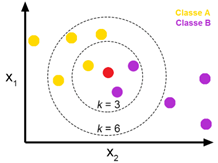
\includegraphics[width=5.5in]{Chap5/KNN.png}
   \caption{KNN}
   \label{fig:KNN}
\end{figure}

\begin{figure}[h]
   \centering
   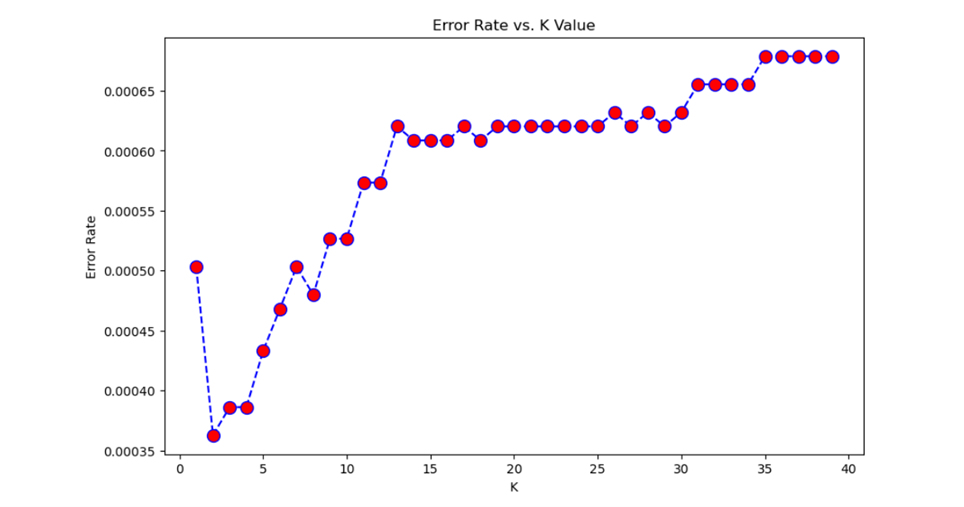
\includegraphics[width=5.5in]{Chap5/Error rate.png}
   \caption{Error Rate}
   \label{fig:Error reate vs K value}
\end{figure}

\begin{figure}[h]
   \centering
   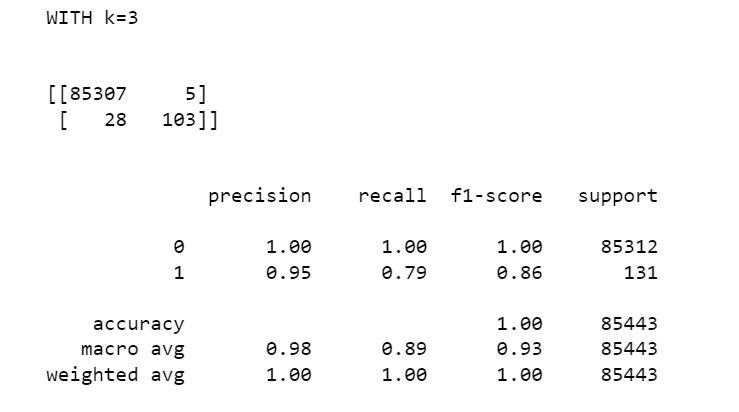
\includegraphics[width=5.5in]{Chap5/K=3.png}
   \caption{K=3}
   \label{fig: K=3}
\end{figure}

Two Ks were used to determine the best KNN model, K=3 and K =7.

•	K = 3
While making the KNN model, We created two models: K =3 and K =7. Figure 5 shows the model created in Jupiter Notebook; the model scored an accuracy of 100\% and identified 85,443 transactions correctly and missed 131. 



•	K = 7


There was a slight decrease in the Accuracy of the model created in Jupiter Notebook (Figure 6) as it scored 100\% when K is 7, and the model miss classified 131 fraudulent transactions as no fraudulent. As for the Accuracy is the same as K=3 100\% with 52 misclassified transactions; the only difference is within the classifications.

\begin{figure}[h]
   \centering
   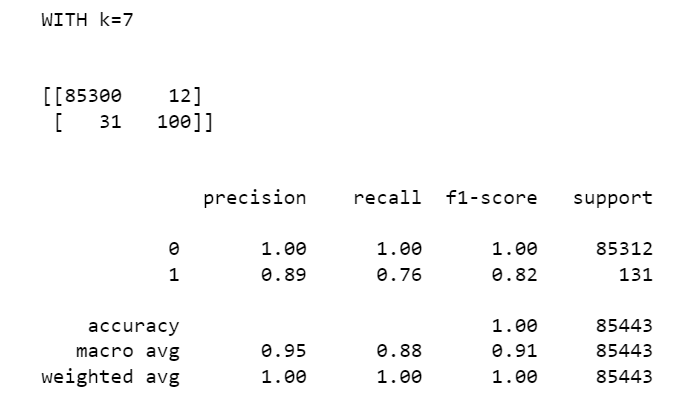
\includegraphics[width=5.5in]{Chap5/K=7.png}
   \caption{K=7}
   \label{fig: K=7}
\end{figure}


\section{Logistic Regression (L.R.):}
This statistical classification model based on probabilities detects Fraud using a logistic curve. Since the value of this logistic curve varies from 0 to 1, it can be used to interpret class membership probabilities. The dataset fed as input to the model is classified for training and testing the model. Post-model activity is tested for some minimum threshold cut-off value for prediction. Based on some threshold probabilities, the logistic Regression can divide the plane using a single line and divide dataset points into exactly two regions.

\begin{figure}[h]
   \centering
   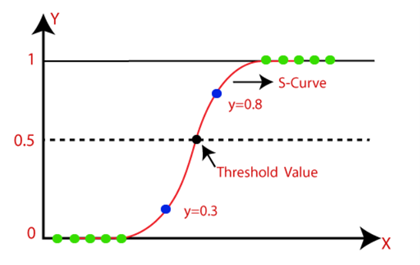
\includegraphics[width=5 in]{Chap5/Logistic Regression.png}
   \caption{Logistic Regression Model}
   \label{fig: Logistic Regression Model}
\end{figure}

The last model created using Jupiter Notebook is Logistic Regression; the model managed to score an Accuracy on Training data of 93.51\% , while it scored an Accuracy score on Test Data of 91.88\%, as presented in  blew Figure.

\begin{figure}[h]
   \centering
   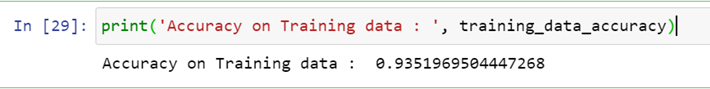
\includegraphics[width=5 in]{Chap5/Train.png}
   \caption{Accuracy on Train data}
   \label{fig: Accuracy on Train data}
\end{figure}


\begin{figure}[h]
   \centering
   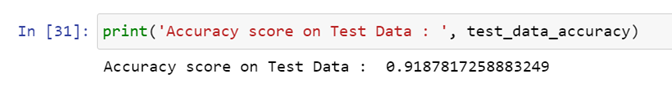
\includegraphics[width=5 in]{Chap5/Test.png}
   \caption{Accuracy on Test data }
   \label{fig:Accuracy on Test data }
\end{figure}

\section{Support Vector Machine (SVM):}
Support vector machines or SVMs are linear classifiers, as stated in that work in high dimensionality because, in high dimensions, a non-linear task in input becomes linear. Hence, this makes SVMs highly useful for detecting Fraud. Its two most important features that is a kernel function to represent the classification function in the dot product of input data point projection and the fact that it tries finding a hyperplane to maximize separation between classes while minimizing overfitting of training data; it provides a very high generalization capability.

\begin{figure}[h]
   \centering
   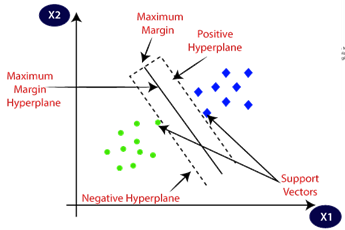
\includegraphics[width=5 in]{Chap5/SVM Algo.png}
   \caption{Support Vector Machine Algorithm}
   \label{fig: Support Vector Machine Algorithm }
\end{figure}

Finally, the model Support Vector Machine, as shown in Figure 12, scored 97.59\% for the Accuracy.

\begin{figure}[h]
   \centering
   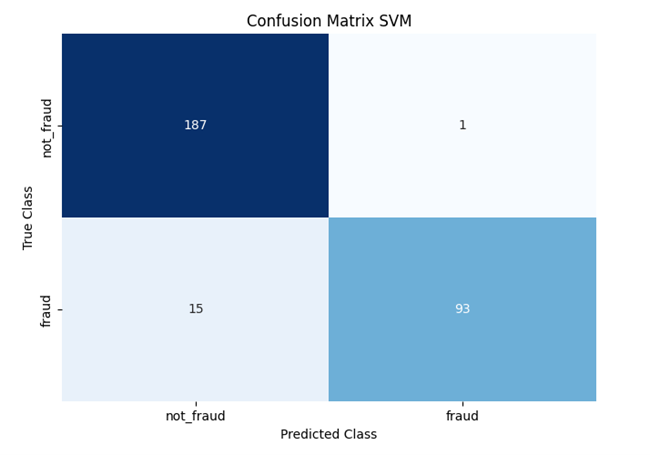
\includegraphics[width=5 in]{Chap5/SVM conf.png}
   \caption{SVM Confusion Matrix}
   \label{fig:SVM Confusion Matrix }
\end{figure}

\begin{figure}[h]
   \centering
   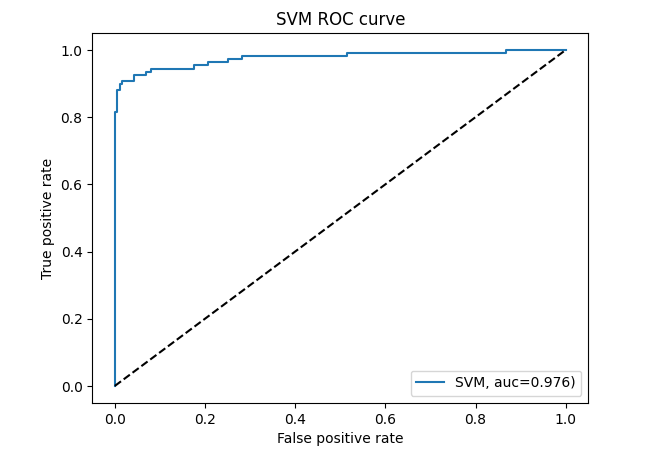
\includegraphics[width=5 in]{Chap5/SVM ROC Curve.png}
   \caption{SVM ROC Curve}
   \label{fig:SVM ROC Curve }
\end{figure}

\section{Decision Tree (D.T.):}
A supervised learning algorithm is a decision tree in the form of a tree structure consisting of the root node and other nodes split in a binary or multi-split manner further into child nodes, with each tree using its algorithm to perform the splitting process. With the tree growing, there may be possibilities of overfitting the training data with possible anomalies in branches, some errors or noise. Hence, pruning is used for improving classification performance of the tree by removing specific nodes. Ease in use and the flexibility that the decision trees provide to handle different data types of attributes make them quite popular.

\begin{figure}[h]
   \centering
   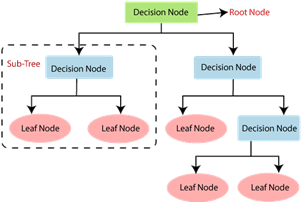
\includegraphics[width=5 in]{Chap5/DT Algo.png}
   \caption{Decision Tree Algorithm}
   \label{fig:Decision Tree Algorithm}
\end{figure}

\textbf{Algorithm: of Decision Tree}
\begin{itemize}
    \item 	Create (T)
    \item 	Calculate frequencies (Ci, T)
    \item   If all instances belong to the same class, the returning leaf
     \item for every Attribute, a test is set for splitting criteria. An attribute that satisfies the test is test node K
    \item Repeating Create (Ti) on each partition Ti.Adding those nodes as children of node K
\end{itemize}


\begin{figure}[h]
   \centering
   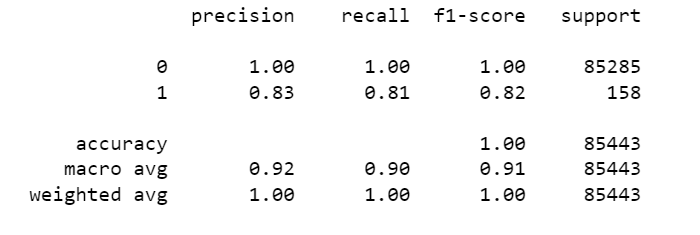
\includegraphics[width=5 in]{Chap5/DT Accuracy.png}
   \caption{D.T. Accuracy}
   \label{fig:D.T. Accuracy}
\end{figure}

\begin{figure}[h]
   \centering
   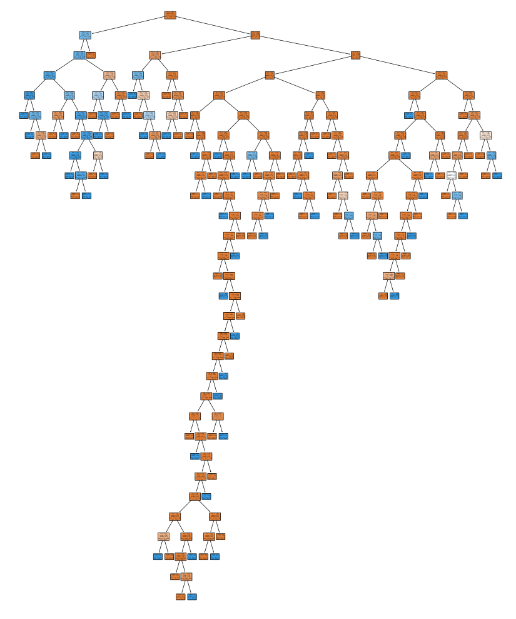
\includegraphics[width=5 in]{Chap5/DT Tree.png}
   \caption{Decision Tree}
   \label{fig:Decision Tree }
\end{figure}


\section{Evaluation and Deployment}
The last stage of the CRISP-DM model is the evaluation and deployment stage, as presented in Table 2 below. All models are being compared to determine the best model for identifying fraudulent credit card transactions.
Accuracy is the overall number of instances that are predicted correctly; accuracies are represented by a confusion matrix where it shows the True Positive (T.P.), True Negative (T.N.), False Positive (F.P.) and False Negative (F.N.). True Positive represents the transactions that are fraudulent and were correctly classified by the model as fraudulent. True Negative represents the not fraudulent transactions that the model correctly predicted as not fraudulent. The third rating is False positive, which represents the fraudulent transaction but was misclassified as not fraudulent. Moreover, finally, False Negative, which are the not fraudulent transactions identified as fraudulent; Table 1 below shows the confusion matrix.


\begin{figure}[h]
   \centering
   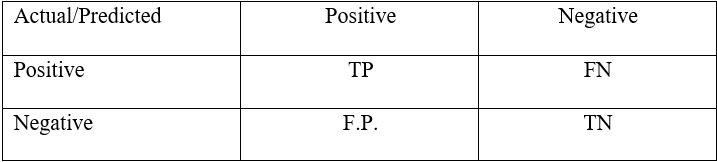
\includegraphics[width=5 in]{Chap5/table.JPG}
   \caption{Confusion Matrix}
   \label{fig:Confusion Matrix-2 }
\end{figure}

The table above shows all the components to calculate the Accuracy of a model, which is displayed in the below equation.

 \begin{figure}[h]
   \centering
   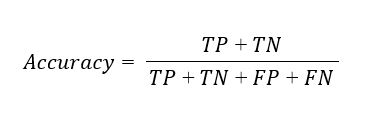
\includegraphics[width=5 in]{Chap5/Conf_Law.JPG}
\end{figure}

\begin{figure}[h]
   \centering
   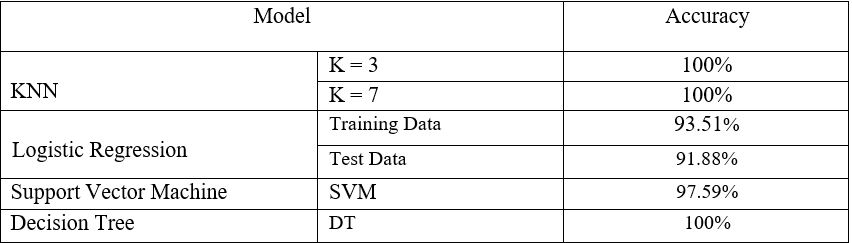
\includegraphics[width=5 in]{Chap5/table2.JPG}
   \caption{Table of Accuracy}
   \label{fig:Table of Accuracy }
\end{figure}

Table 2 shows all of the accuracies of all the models that were created in the project; all models performed well in detecting fraudulent transactions and managed to score high accuracies. Out of all the models, the model that scored the best is KNN and Decision Tree as its Accuracy is 100\%, the third place is the Support Vector Machine, and the model that scored the lowest Accuracy out of all models is Logistic Regression with a score of 93.51\%.



